\documentclass[1p]{elsarticle_modified}
%\bibliographystyle{elsarticle-num}

%\usepackage[colorlinks]{hyperref}
%\usepackage{abbrmath_seonhwa} %\Abb, \Ascr, \Acal ,\Abf, \Afrak
\usepackage{amsfonts}
\usepackage{amssymb}
\usepackage{amsmath}
\usepackage{amsthm}
\usepackage{scalefnt}
\usepackage{amsbsy}
\usepackage{kotex}
\usepackage{caption}
\usepackage{subfig}
\usepackage{color}
\usepackage{graphicx}
\usepackage{xcolor} %% white, black, red, green, blue, cyan, magenta, yellow
\usepackage{float}
\usepackage{setspace}
\usepackage{hyperref}

\usepackage{tikz}
\usetikzlibrary{arrows}

\usepackage{multirow}
\usepackage{array} % fixed length table
\usepackage{hhline}

%%%%%%%%%%%%%%%%%%%%%
\makeatletter
\renewcommand*\env@matrix[1][\arraystretch]{%
	\edef\arraystretch{#1}%
	\hskip -\arraycolsep
	\let\@ifnextchar\new@ifnextchar
	\array{*\c@MaxMatrixCols c}}
\makeatother %https://tex.stackexchange.com/questions/14071/how-can-i-increase-the-line-spacing-in-a-matrix
%%%%%%%%%%%%%%%

\usepackage[normalem]{ulem}

\newcommand{\msout}[1]{\ifmmode\text{\sout{\ensuremath{#1}}}\else\sout{#1}\fi}
%SOURCE: \msout is \stkout macro in https://tex.stackexchange.com/questions/20609/strikeout-in-math-mode

\newcommand{\cancel}[1]{
	\ifmmode
	{\color{red}\msout{#1}}
	\else
	{\color{red}\sout{#1}}
	\fi
}

\newcommand{\add}[1]{
	{\color{blue}\uwave{#1}}
}

\newcommand{\replace}[2]{
	\ifmmode
	{\color{red}\msout{#1}}{\color{blue}\uwave{#2}}
	\else
	{\color{red}\sout{#1}}{\color{blue}\uwave{#2}}
	\fi
}

\newcommand{\Sol}{\mathcal{S}} %segment
\newcommand{\D}{D} %diagram
\newcommand{\A}{\mathcal{A}} %arc


%%%%%%%%%%%%%%%%%%%%%%%%%%%%%5 test

\def\sl{\operatorname{\textup{SL}}(2,\Cbb)}
\def\psl{\operatorname{\textup{PSL}}(2,\Cbb)}
\def\quan{\mkern 1mu \triangleright \mkern 1mu}

\theoremstyle{definition}
\newtheorem{thm}{Theorem}[section]
\newtheorem{prop}[thm]{Proposition}
\newtheorem{lem}[thm]{Lemma}
\newtheorem{ques}[thm]{Question}
\newtheorem{cor}[thm]{Corollary}
\newtheorem{defn}[thm]{Definition}
\newtheorem{exam}[thm]{Example}
\newtheorem{rmk}[thm]{Remark}
\newtheorem{alg}[thm]{Algorithm}

\newcommand{\I}{\sqrt{-1}}
\begin{document}

%\begin{frontmatter}
%
%\title{Boundary parabolic representations of knots up to 8 crossings}
%
%%% Group authors per affiliation:
%\author{Yunhi Cho} 
%\address{Department of Mathematics, University of Seoul, Seoul, Korea}
%\ead{yhcho@uos.ac.kr}
%
%
%\author{Seonhwa Kim} %\fnref{s_kim}}
%\address{Center for Geometry and Physics, Institute for Basic Science, Pohang, 37673, Korea}
%\ead{ryeona17@ibs.re.kr}
%
%\author{Hyuk Kim}
%\address{Department of Mathematical Sciences, Seoul National University, Seoul 08826, Korea}
%\ead{hyukkim@snu.ac.kr}
%
%\author{Seokbeom Yoon}
%\address{Department of Mathematical Sciences, Seoul National University, Seoul, 08826,  Korea}
%\ead{sbyoon15@snu.ac.kr}
%
%\begin{abstract}
%We find all boundary parabolic representation of knots up to 8 crossings.
%
%\end{abstract}
%\begin{keyword}
%    \MSC[2010] 57M25 
%\end{keyword}
%
%\end{frontmatter}

%\linenumbers
%\tableofcontents
%
\newcommand\colored[1]{\textcolor{white}{\rule[-0.35ex]{0.8em}{1.4ex}}\kern-0.8em\color{red} #1}%
%\newcommand\colored[1]{\textcolor{white}{ #1}\kern-2.17ex	\textcolor{white}{ #1}\kern-1.81ex	\textcolor{white}{ #1}\kern-2.15ex\color{red}#1	}

{\Large $\underline{11n_{24}~(K11n_{24})}$}

\setlength{\tabcolsep}{10pt}
\renewcommand{\arraystretch}{1.6}
\vspace{1cm}\begin{tabular}{m{100pt}>{\centering\arraybackslash}m{274pt}}
\multirow{5}{120pt}{
	\centering
	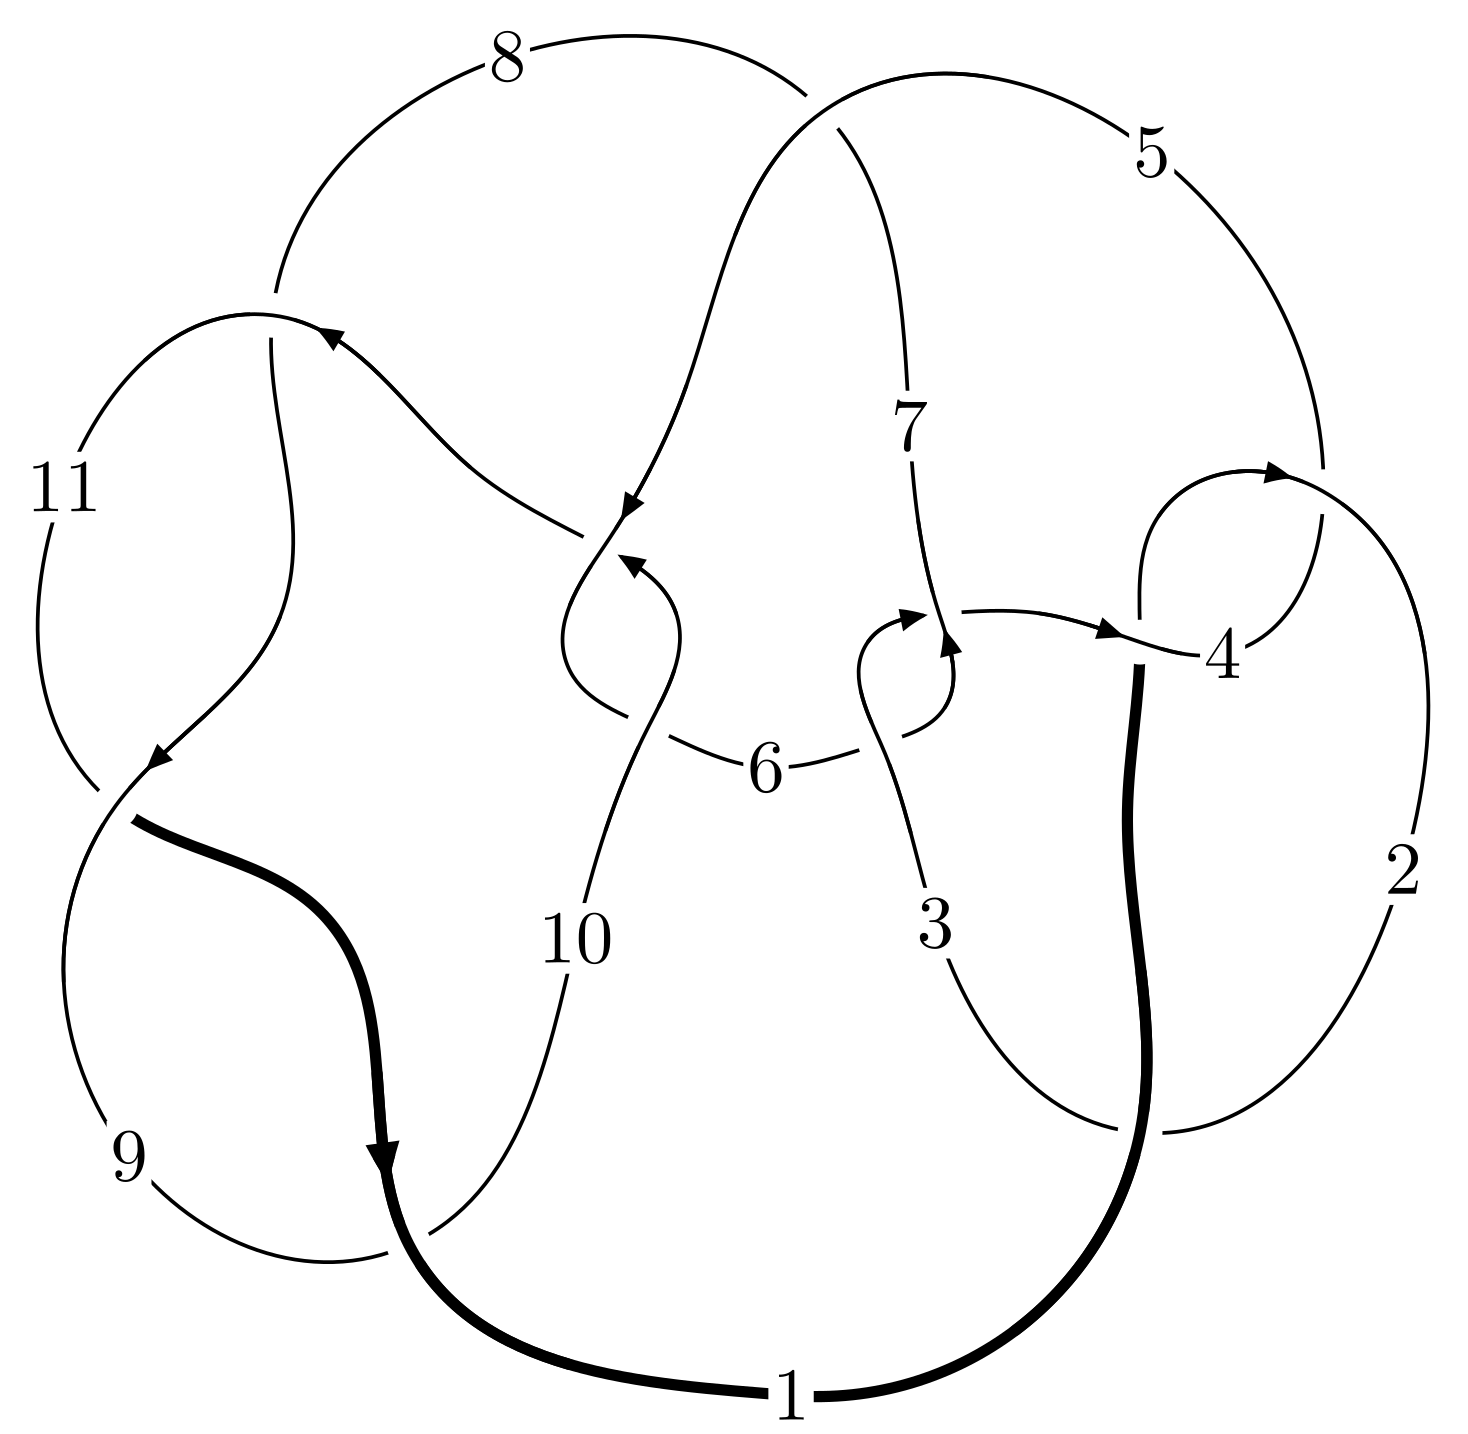
\includegraphics[width=112pt]{../../../GIT/diagram.site/Diagrams/png/640_11n_24.png}\\
\ \ \ A knot diagram\footnotemark}&
\allowdisplaybreaks
\textbf{Linearized knot diagam} \\
\cline{2-2}
 &
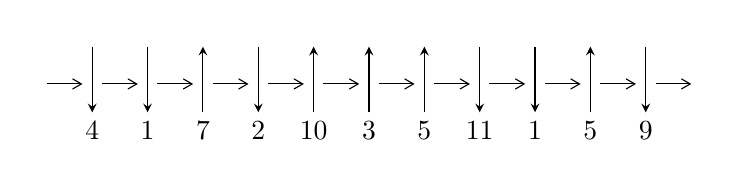
\begin{tikzpicture}[x=20pt, y=17pt]
	% nodes
	\node (C0) at (0, 0) {};
	\node (C1) at (1, 0) {};
	\node (C1U) at (1, +1) {};
	\node (C1D) at (1, -1) {4};

	\node (C2) at (2, 0) {};
	\node (C2U) at (2, +1) {};
	\node (C2D) at (2, -1) {1};

	\node (C3) at (3, 0) {};
	\node (C3U) at (3, +1) {};
	\node (C3D) at (3, -1) {7};

	\node (C4) at (4, 0) {};
	\node (C4U) at (4, +1) {};
	\node (C4D) at (4, -1) {2};

	\node (C5) at (5, 0) {};
	\node (C5U) at (5, +1) {};
	\node (C5D) at (5, -1) {10};

	\node (C6) at (6, 0) {};
	\node (C6U) at (6, +1) {};
	\node (C6D) at (6, -1) {3};

	\node (C7) at (7, 0) {};
	\node (C7U) at (7, +1) {};
	\node (C7D) at (7, -1) {5};

	\node (C8) at (8, 0) {};
	\node (C8U) at (8, +1) {};
	\node (C8D) at (8, -1) {11};

	\node (C9) at (9, 0) {};
	\node (C9U) at (9, +1) {};
	\node (C9D) at (9, -1) {1};

	\node (C10) at (10, 0) {};
	\node (C10U) at (10, +1) {};
	\node (C10D) at (10, -1) {5};

	\node (C11) at (11, 0) {};
	\node (C11U) at (11, +1) {};
	\node (C11D) at (11, -1) {9};
	\node (C12) at (12, 0) {};

	% arrows
	\draw[->,>={angle 60}]
	(C0) edge (C1) (C1) edge (C2) (C2) edge (C3) (C3) edge (C4) (C4) edge (C5) (C5) edge (C6) (C6) edge (C7) (C7) edge (C8) (C8) edge (C9) (C9) edge (C10) (C10) edge (C11) (C11) edge (C12) ;	\draw[->,>=stealth]
	(C1U) edge (C1D) (C2U) edge (C2D) (C3D) edge (C3U) (C4U) edge (C4D) (C5D) edge (C5U) (C6D) edge (C6U) (C7D) edge (C7U) (C8U) edge (C8D) (C9U) edge (C9D) (C10D) edge (C10U) (C11U) edge (C11D) ;
	\end{tikzpicture} \\
\hhline{~~} \\& 
\textbf{Solving Sequence} \\ \cline{2-2} 
 &
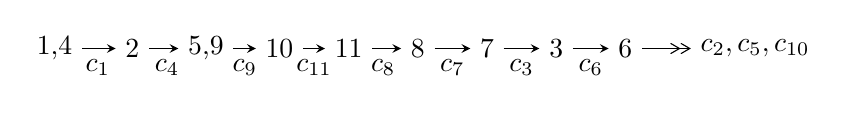
\begin{tikzpicture}[x=25pt, y=7pt]
	% node
	\node (A0) at (-1/8, 0) {1,4};
	\node (A1) at (1, 0) {2};
	\node (A2) at (33/16, 0) {5,9};
	\node (A3) at (25/8, 0) {10};
	\node (A4) at (33/8, 0) {11};
	\node (A5) at (41/8, 0) {8};
	\node (A6) at (49/8, 0) {7};
	\node (A7) at (57/8, 0) {3};
	\node (A8) at (65/8, 0) {6};
	\node (C1) at (1/2, -1) {$c_{1}$};
	\node (C2) at (3/2, -1) {$c_{4}$};
	\node (C3) at (21/8, -1) {$c_{9}$};
	\node (C4) at (29/8, -1) {$c_{11}$};
	\node (C5) at (37/8, -1) {$c_{8}$};
	\node (C6) at (45/8, -1) {$c_{7}$};
	\node (C7) at (53/8, -1) {$c_{3}$};
	\node (C8) at (61/8, -1) {$c_{6}$};
	\node (A9) at (10, 0) {$c_{2},c_{5},c_{10}$};

	% edge
	\draw[->,>=stealth]	
	(A0) edge (A1) (A1) edge (A2) (A2) edge (A3) (A3) edge (A4) (A4) edge (A5) (A5) edge (A6) (A6) edge (A7) (A7) edge (A8) ;
	\draw[->>,>={angle 60}]	
	(A8) edge (A9);
\end{tikzpicture} \\ 

\end{tabular} \\

\footnotetext{
The image of knot diagram is generated by the software ``\textbf{Draw programme}" developed by Andrew Bartholomew(\url{http://www.layer8.co.uk/maths/draw/index.htm\#Running-draw}), where we modified some parts for our purpose(\url{https://github.com/CATsTAILs/LinksPainter}).
}\phantom \\ \newline 
\centering \textbf{Ideals for irreducible components\footnotemark of $X_{\text{par}}$} 
 
\begin{align*}
I^u_{1}&=\langle 
-44 u^{16}+153 u^{15}+\cdots+4229 b+2570,\;-15 u^{16}+2455 u^{15}+\cdots+4229 a-4314,\\
\phantom{I^u_{1}}&\phantom{= \langle  }u^{17}+2 u^{16}+\cdots+u-1\rangle \\
I^u_{2}&=\langle 
b+1,\;- u^4- u^3+a+u+1,\;u^6+u^5- u^4-2 u^3+u+1\rangle \\
\\
\end{align*}
\raggedright * 2 irreducible components of $\dim_{\mathbb{C}}=0$, with total 23 representations.\\
\footnotetext{All coefficients of polynomials are rational numbers. But the coefficients are sometimes approximated in decimal forms when there is not enough margin.}
\newpage
\renewcommand{\arraystretch}{1}
\centering \section*{I. $I^u_{1}= \langle -44 u^{16}+153 u^{15}+\cdots+4229 b+2570,\;-15 u^{16}+2455 u^{15}+\cdots+4229 a-4314,\;u^{17}+2 u^{16}+\cdots+u-1 \rangle$}
\flushleft \textbf{(i) Arc colorings}\\
\begin{tabular}{m{7pt} m{180pt} m{7pt} m{180pt} }
\flushright $a_{1}=$&$\begin{pmatrix}1\\0\end{pmatrix}$ \\
\flushright $a_{4}=$&$\begin{pmatrix}0\\u\end{pmatrix}$ \\
\flushright $a_{2}=$&$\begin{pmatrix}1\\u^2\end{pmatrix}$ \\
\flushright $a_{5}=$&$\begin{pmatrix}- u\\- u^3+u\end{pmatrix}$ \\
\flushright $a_{9}=$&$\begin{pmatrix}0.00354694 u^{16}-0.580515 u^{15}+\cdots+1.76046 u+1.02010\\0.0104044 u^{16}-0.0361788 u^{15}+\cdots-1.16931 u-0.607709\end{pmatrix}$ \\
\flushright $a_{10}=$&$\begin{pmatrix}-0.00685741 u^{16}-0.544337 u^{15}+\cdots+2.92977 u+1.62781\\0.0104044 u^{16}-0.0361788 u^{15}+\cdots-1.16931 u-0.607709\end{pmatrix}$ \\
\flushright $a_{11}=$&$\begin{pmatrix}-0.0245921 u^{16}-0.641759 u^{15}+\cdots+3.12745 u+1.52731\\-0.0416174 u^{16}+0.144715 u^{15}+\cdots-1.32277 u-0.569165\end{pmatrix}$ \\
\flushright $a_{8}=$&$\begin{pmatrix}0.933318 u^{16}+0.913691 u^{15}+\cdots-2.09671 u-0.377867\\0.895956 u^{16}+0.361788 u^{15}+\cdots+1.69307 u-0.922913\end{pmatrix}$ \\
\flushright $a_{7}=$&$\begin{pmatrix}-0.0134784 u^{16}+0.205959 u^{15}+\cdots-2.68976 u-0.0763774\\0.0520218 u^{16}-0.180894 u^{15}+\cdots+0.153464 u-0.0385434\end{pmatrix}$ \\
\flushright $a_{3}=$&$\begin{pmatrix}- u^2+1\\u^2\end{pmatrix}$ \\
\flushright $a_{6}=$&$\begin{pmatrix}-0.0300307 u^{16}+0.581698 u^{15}+\cdots-3.23859 u+0.163159\\0.301490 u^{16}-0.343817 u^{15}+\cdots+0.639395 u-0.291558\end{pmatrix}$\\ \flushright $a_{6}=$&$\begin{pmatrix}-0.0300307 u^{16}+0.581698 u^{15}+\cdots-3.23859 u+0.163159\\0.301490 u^{16}-0.343817 u^{15}+\cdots+0.639395 u-0.291558\end{pmatrix}$\\&\end{tabular}
\flushleft \textbf{(ii) Obstruction class $= -1$}\\~\\
\flushleft \textbf{(iii) Cusp Shapes $= \frac{7665}{4229} u^{16}+\frac{5737}{4229} u^{15}+\cdots-\frac{1705}{4229} u-\frac{11542}{4229}$}\\~\\
\newpage\renewcommand{\arraystretch}{1}
\flushleft \textbf{(iv) u-Polynomials at the component}\newline \\
\begin{tabular}{m{50pt}|m{274pt}}
Crossings & \hspace{64pt}u-Polynomials at each crossing \\
\hline $$\begin{aligned}c_{1},c_{4}\end{aligned}$$&$\begin{aligned}
&u^{17}-2 u^{16}+\cdots+u+1
\end{aligned}$\\
\hline $$\begin{aligned}c_{2}\end{aligned}$$&$\begin{aligned}
&u^{17}+12 u^{16}+\cdots- u+1
\end{aligned}$\\
\hline $$\begin{aligned}c_{3},c_{6}\end{aligned}$$&$\begin{aligned}
&u^{17}-2 u^{16}+\cdots+u-1
\end{aligned}$\\
\hline $$\begin{aligned}c_{5},c_{10}\end{aligned}$$&$\begin{aligned}
&u^{17}+3 u^{16}+\cdots+128 u-64
\end{aligned}$\\
\hline $$\begin{aligned}c_{7}\end{aligned}$$&$\begin{aligned}
&u^{17}+6 u^{16}+\cdots+3897 u+1609
\end{aligned}$\\
\hline $$\begin{aligned}c_{8},c_{9},c_{11}\end{aligned}$$&$\begin{aligned}
&u^{17}-7 u^{16}+\cdots+18 u^2+1
\end{aligned}$\\
\hline
\end{tabular}\\~\\
\newpage\renewcommand{\arraystretch}{1}
\flushleft \textbf{(v) Riley Polynomials at the component}\newline \\
\begin{tabular}{m{50pt}|m{274pt}}
Crossings & \hspace{64pt}Riley Polynomials at each crossing \\
\hline $$\begin{aligned}c_{1},c_{4}\end{aligned}$$&$\begin{aligned}
&y^{17}-12 y^{16}+\cdots- y-1
\end{aligned}$\\
\hline $$\begin{aligned}c_{2}\end{aligned}$$&$\begin{aligned}
&y^{17}-12 y^{16}+\cdots-77 y-1
\end{aligned}$\\
\hline $$\begin{aligned}c_{3},c_{6}\end{aligned}$$&$\begin{aligned}
&y^{17}+18 y^{15}+\cdots- y-1
\end{aligned}$\\
\hline $$\begin{aligned}c_{5},c_{10}\end{aligned}$$&$\begin{aligned}
&y^{17}+39 y^{16}+\cdots+8192 y-4096
\end{aligned}$\\
\hline $$\begin{aligned}c_{7}\end{aligned}$$&$\begin{aligned}
&y^{17}+68 y^{16}+\cdots-35776857 y-2588881
\end{aligned}$\\
\hline $$\begin{aligned}c_{8},c_{9},c_{11}\end{aligned}$$&$\begin{aligned}
&y^{17}-31 y^{16}+\cdots-36 y-1
\end{aligned}$\\
\hline
\end{tabular}\\~\\
\newpage\flushleft \textbf{(vi) Complex Volumes and Cusp Shapes}
$$\begin{array}{c|c|c}  
\text{Solutions to }I^u_{1}& \I (\text{vol} + \sqrt{-1}CS) & \text{Cusp shape}\\
 \hline 
\begin{aligned}
u &= \phantom{-}0.977894 + 0.194640 I \\
a &= \phantom{-}0.644273 + 0.271764 I \\
b &= -0.074423 - 0.157594 I\end{aligned}
 & -1.75571 - 0.69092 I & -4.20927 - 0.03881 I \\ \hline\begin{aligned}
u &= \phantom{-}0.977894 - 0.194640 I \\
a &= \phantom{-}0.644273 - 0.271764 I \\
b &= -0.074423 + 0.157594 I\end{aligned}
 & -1.75571 + 0.69092 I & -4.20927 + 0.03881 I \\ \hline\begin{aligned}
u &= \phantom{-}0.007198 + 1.101270 I \\
a &= \phantom{-}0.0948459 - 0.0860640 I \\
b &= \phantom{-}2.00423 + 0.17609 I\end{aligned}
 & -14.0076 - 4.0781 I & -2.81048 + 2.03189 I \\ \hline\begin{aligned}
u &= \phantom{-}0.007198 - 1.101270 I \\
a &= \phantom{-}0.0948459 + 0.0860640 I \\
b &= \phantom{-}2.00423 - 0.17609 I\end{aligned}
 & -14.0076 + 4.0781 I & -2.81048 - 2.03189 I \\ \hline\begin{aligned}
u &= \phantom{-}1.11899\phantom{ +0.000000I} \\
a &= -3.55652\phantom{ +0.000000I} \\
b &= -1.14890\phantom{ +0.000000I}\end{aligned}
 & -3.74765\phantom{ +0.000000I} & \phantom{-}10.6760\phantom{ +0.000000I} \\ \hline\begin{aligned}
u &= -1.094410 + 0.448256 I \\
a &= \phantom{-}0.297387 + 0.400102 I \\
b &= \phantom{-}0.394810 + 0.688088 I\end{aligned}
 & -0.57451 + 4.58866 I & -0.38155 - 5.05474 I \\ \hline\begin{aligned}
u &= -1.094410 - 0.448256 I \\
a &= \phantom{-}0.297387 - 0.400102 I \\
b &= \phantom{-}0.394810 - 0.688088 I\end{aligned}
 & -0.57451 - 4.58866 I & -0.38155 + 5.05474 I \\ \hline\begin{aligned}
u &= -1.279610 + 0.127778 I \\
a &= -1.75394 + 0.15484 I \\
b &= -1.65978 + 0.99674 I\end{aligned}
 & -6.36531 + 2.55518 I & -9.15621 - 3.45666 I \\ \hline\begin{aligned}
u &= -1.279610 - 0.127778 I \\
a &= -1.75394 - 0.15484 I \\
b &= -1.65978 - 0.99674 I\end{aligned}
 & -6.36531 - 2.55518 I & -9.15621 + 3.45666 I \\ \hline\begin{aligned}
u &= -0.397422 + 0.534657 I \\
a &= \phantom{-}0.841166 + 0.259861 I \\
b &= \phantom{-}0.289585 - 0.225601 I\end{aligned}
 & \phantom{-}1.46199 - 0.53067 I & \phantom{-}6.34861 + 0.44801 I\\
 \hline 
 \end{array}$$\newpage$$\begin{array}{c|c|c}  
\text{Solutions to }I^u_{1}& \I (\text{vol} + \sqrt{-1}CS) & \text{Cusp shape}\\
 \hline 
\begin{aligned}
u &= -0.397422 - 0.534657 I \\
a &= \phantom{-}0.841166 - 0.259861 I \\
b &= \phantom{-}0.289585 + 0.225601 I\end{aligned}
 & \phantom{-}1.46199 + 0.53067 I & \phantom{-}6.34861 - 0.44801 I \\ \hline\begin{aligned}
u &= -1.38093 + 0.53931 I \\
a &= \phantom{-}1.72060 + 1.08326 I \\
b &= \phantom{-}2.05747 - 0.40594 I\end{aligned}
 & -18.3559 + 9.9055 I & -5.27294 - 4.68483 I \\ \hline\begin{aligned}
u &= -1.38093 - 0.53931 I \\
a &= \phantom{-}1.72060 - 1.08326 I \\
b &= \phantom{-}2.05747 + 0.40594 I\end{aligned}
 & -18.3559 - 9.9055 I & -5.27294 + 4.68483 I \\ \hline\begin{aligned}
u &= \phantom{-}1.38223 + 0.54918 I \\
a &= \phantom{-}1.50860 - 1.17337 I \\
b &= \phantom{-}2.09111 + 0.05760 I\end{aligned}
 & -18.3031 - 1.7986 I & -5.37966 + 0.73401 I \\ \hline\begin{aligned}
u &= \phantom{-}1.38223 - 0.54918 I \\
a &= \phantom{-}1.50860 + 1.17337 I \\
b &= \phantom{-}2.09111 - 0.05760 I\end{aligned}
 & -18.3031 + 1.7986 I & -5.37966 - 0.73401 I \\ \hline\begin{aligned}
u &= \phantom{-}0.225548 + 0.312459 I \\
a &= \phantom{-}1.92533 + 0.42540 I \\
b &= -1.028560 - 0.314868 I\end{aligned}
 & -1.91105 - 0.93427 I & -3.47646 + 1.18545 I \\ \hline\begin{aligned}
u &= \phantom{-}0.225548 - 0.312459 I \\
a &= \phantom{-}1.92533 - 0.42540 I \\
b &= -1.028560 + 0.314868 I\end{aligned}
 & -1.91105 + 0.93427 I & -3.47646 - 1.18545 I\\
 \hline 
 \end{array}$$\newpage\newpage\renewcommand{\arraystretch}{1}
\centering \section*{II. $I^u_{2}= \langle b+1,\;- u^4- u^3+a+u+1,\;u^6+u^5- u^4-2 u^3+u+1 \rangle$}
\flushleft \textbf{(i) Arc colorings}\\
\begin{tabular}{m{7pt} m{180pt} m{7pt} m{180pt} }
\flushright $a_{1}=$&$\begin{pmatrix}1\\0\end{pmatrix}$ \\
\flushright $a_{4}=$&$\begin{pmatrix}0\\u\end{pmatrix}$ \\
\flushright $a_{2}=$&$\begin{pmatrix}1\\u^2\end{pmatrix}$ \\
\flushright $a_{5}=$&$\begin{pmatrix}- u\\- u^3+u\end{pmatrix}$ \\
\flushright $a_{9}=$&$\begin{pmatrix}u^4+u^3- u-1\\-1\end{pmatrix}$ \\
\flushright $a_{10}=$&$\begin{pmatrix}u^4+u^3- u\\-1\end{pmatrix}$ \\
\flushright $a_{11}=$&$\begin{pmatrix}u^4+u^3- u\\-1\end{pmatrix}$ \\
\flushright $a_{8}=$&$\begin{pmatrix}-1\\0\end{pmatrix}$ \\
\flushright $a_{7}=$&$\begin{pmatrix}- u^4+u^2-1\\u^5+u^4-2 u^3- u^2+u+1\end{pmatrix}$ \\
\flushright $a_{3}=$&$\begin{pmatrix}- u^2+1\\u^2\end{pmatrix}$ \\
\flushright $a_{6}=$&$\begin{pmatrix}- u\\- u^3+u\end{pmatrix}$\\ \flushright $a_{6}=$&$\begin{pmatrix}- u\\- u^3+u\end{pmatrix}$\\&\end{tabular}
\flushleft \textbf{(ii) Obstruction class $= 1$}\\~\\
\flushleft \textbf{(iii) Cusp Shapes $= 3 u^4-2 u^3-3 u^2-2 u-1$}\\~\\
\newpage\renewcommand{\arraystretch}{1}
\flushleft \textbf{(iv) u-Polynomials at the component}\newline \\
\begin{tabular}{m{50pt}|m{274pt}}
Crossings & \hspace{64pt}u-Polynomials at each crossing \\
\hline $$\begin{aligned}c_{1},c_{6}\end{aligned}$$&$\begin{aligned}
&u^6+u^5- u^4-2 u^3+u+1
\end{aligned}$\\
\hline $$\begin{aligned}c_{2}\end{aligned}$$&$\begin{aligned}
&u^6+3 u^5+5 u^4+4 u^3+2 u^2+u+1
\end{aligned}$\\
\hline $$\begin{aligned}c_{3},c_{4}\end{aligned}$$&$\begin{aligned}
&u^6- u^5- u^4+2 u^3- u+1
\end{aligned}$\\
\hline $$\begin{aligned}c_{5},c_{10}\end{aligned}$$&$\begin{aligned}
&u^6
\end{aligned}$\\
\hline $$\begin{aligned}c_{7}\end{aligned}$$&$\begin{aligned}
&u^6-3 u^5+5 u^4-4 u^3+2 u^2- u+1
\end{aligned}$\\
\hline $$\begin{aligned}c_{8},c_{9}\end{aligned}$$&$\begin{aligned}
&(u-1)^6
\end{aligned}$\\
\hline $$\begin{aligned}c_{11}\end{aligned}$$&$\begin{aligned}
&(u+1)^6
\end{aligned}$\\
\hline
\end{tabular}\\~\\
\newpage\renewcommand{\arraystretch}{1}
\flushleft \textbf{(v) Riley Polynomials at the component}\newline \\
\begin{tabular}{m{50pt}|m{274pt}}
Crossings & \hspace{64pt}Riley Polynomials at each crossing \\
\hline $$\begin{aligned}c_{1},c_{3},c_{4}\\c_{6}\end{aligned}$$&$\begin{aligned}
&y^6-3 y^5+5 y^4-4 y^3+2 y^2- y+1
\end{aligned}$\\
\hline $$\begin{aligned}c_{2},c_{7}\end{aligned}$$&$\begin{aligned}
&y^6+y^5+5 y^4+6 y^2+3 y+1
\end{aligned}$\\
\hline $$\begin{aligned}c_{5},c_{10}\end{aligned}$$&$\begin{aligned}
&y^6
\end{aligned}$\\
\hline $$\begin{aligned}c_{8},c_{9},c_{11}\end{aligned}$$&$\begin{aligned}
&(y-1)^6
\end{aligned}$\\
\hline
\end{tabular}\\~\\
\newpage\flushleft \textbf{(vi) Complex Volumes and Cusp Shapes}
$$\begin{array}{c|c|c}  
\text{Solutions to }I^u_{2}& \I (\text{vol} + \sqrt{-1}CS) & \text{Cusp shape}\\
 \hline 
\begin{aligned}
u &= \phantom{-}1.002190 + 0.295542 I \\
a &= -0.76815 + 1.65564 I \\
b &= -1.00000\phantom{ +0.000000I}\end{aligned}
 & -3.53554 - 0.92430 I & -5.77331 - 0.83820 I \\ \hline\begin{aligned}
u &= \phantom{-}1.002190 - 0.295542 I \\
a &= -0.76815 - 1.65564 I \\
b &= -1.00000\phantom{ +0.000000I}\end{aligned}
 & -3.53554 + 0.92430 I & -5.77331 + 0.83820 I \\ \hline\begin{aligned}
u &= -0.428243 + 0.664531 I \\
a &= -0.340228 - 0.298454 I \\
b &= -1.00000\phantom{ +0.000000I}\end{aligned}
 & \phantom{-}0.245672 - 0.924305 I & -1.11831 + 1.11590 I \\ \hline\begin{aligned}
u &= -0.428243 - 0.664531 I \\
a &= -0.340228 + 0.298454 I \\
b &= -1.00000\phantom{ +0.000000I}\end{aligned}
 & \phantom{-}0.245672 + 0.924305 I & -1.11831 - 1.11590 I \\ \hline\begin{aligned}
u &= -1.073950 + 0.558752 I \\
a &= -0.891622 - 0.818891 I \\
b &= -1.00000\phantom{ +0.000000I}\end{aligned}
 & -1.64493 + 5.69302 I & -3.10838 - 7.09196 I \\ \hline\begin{aligned}
u &= -1.073950 - 0.558752 I \\
a &= -0.891622 + 0.818891 I \\
b &= -1.00000\phantom{ +0.000000I}\end{aligned}
 & -1.64493 - 5.69302 I & -3.10838 + 7.09196 I\\
 \hline 
 \end{array}$$\newpage
\newpage\renewcommand{\arraystretch}{1}
\centering \section*{ III. u-Polynomials}
\begin{tabular}{m{50pt}|m{274pt}}
Crossings & \hspace{64pt}u-Polynomials at each crossing \\
\hline $$\begin{aligned}c_{1}\end{aligned}$$&$\begin{aligned}
&(u^6+u^5- u^4-2 u^3+u+1)(u^{17}-2 u^{16}+\cdots+u+1)
\end{aligned}$\\
\hline $$\begin{aligned}c_{2}\end{aligned}$$&$\begin{aligned}
&(u^6+3 u^5+5 u^4+4 u^3+2 u^2+u+1)(u^{17}+12 u^{16}+\cdots- u+1)
\end{aligned}$\\
\hline $$\begin{aligned}c_{3}\end{aligned}$$&$\begin{aligned}
&(u^6- u^5- u^4+2 u^3- u+1)(u^{17}-2 u^{16}+\cdots+u-1)
\end{aligned}$\\
\hline $$\begin{aligned}c_{4}\end{aligned}$$&$\begin{aligned}
&(u^6- u^5- u^4+2 u^3- u+1)(u^{17}-2 u^{16}+\cdots+u+1)
\end{aligned}$\\
\hline $$\begin{aligned}c_{5},c_{10}\end{aligned}$$&$\begin{aligned}
&u^6(u^{17}+3 u^{16}+\cdots+128 u-64)
\end{aligned}$\\
\hline $$\begin{aligned}c_{6}\end{aligned}$$&$\begin{aligned}
&(u^6+u^5- u^4-2 u^3+u+1)(u^{17}-2 u^{16}+\cdots+u-1)
\end{aligned}$\\
\hline $$\begin{aligned}c_{7}\end{aligned}$$&$\begin{aligned}
&(u^6-3 u^5+5 u^4-4 u^3+2 u^2- u+1)(u^{17}+6 u^{16}+\cdots+3897 u+1609)
\end{aligned}$\\
\hline $$\begin{aligned}c_{8},c_{9}\end{aligned}$$&$\begin{aligned}
&((u-1)^6)(u^{17}-7 u^{16}+\cdots+18 u^2+1)
\end{aligned}$\\
\hline $$\begin{aligned}c_{11}\end{aligned}$$&$\begin{aligned}
&((u+1)^6)(u^{17}-7 u^{16}+\cdots+18 u^2+1)
\end{aligned}$\\
\hline
\end{tabular}\newpage\renewcommand{\arraystretch}{1}
\centering \section*{ IV. Riley Polynomials}
\begin{tabular}{m{50pt}|m{274pt}}
Crossings & \hspace{64pt}Riley Polynomials at each crossing \\
\hline $$\begin{aligned}c_{1},c_{4}\end{aligned}$$&$\begin{aligned}
&(y^6-3 y^5+5 y^4-4 y^3+2 y^2- y+1)(y^{17}-12 y^{16}+\cdots- y-1)
\end{aligned}$\\
\hline $$\begin{aligned}c_{2}\end{aligned}$$&$\begin{aligned}
&(y^6+y^5+5 y^4+6 y^2+3 y+1)(y^{17}-12 y^{16}+\cdots-77 y-1)
\end{aligned}$\\
\hline $$\begin{aligned}c_{3},c_{6}\end{aligned}$$&$\begin{aligned}
&(y^6-3 y^5+5 y^4-4 y^3+2 y^2- y+1)(y^{17}+18 y^{15}+\cdots- y-1)
\end{aligned}$\\
\hline $$\begin{aligned}c_{5},c_{10}\end{aligned}$$&$\begin{aligned}
&y^6(y^{17}+39 y^{16}+\cdots+8192 y-4096)
\end{aligned}$\\
\hline $$\begin{aligned}c_{7}\end{aligned}$$&$\begin{aligned}
&(y^6+y^5+5 y^4+6 y^2+3 y+1)\\
&\cdot(y^{17}+68 y^{16}+\cdots-35776857 y-2588881)
\end{aligned}$\\
\hline $$\begin{aligned}c_{8},c_{9},c_{11}\end{aligned}$$&$\begin{aligned}
&((y-1)^6)(y^{17}-31 y^{16}+\cdots-36 y-1)
\end{aligned}$\\
\hline
\end{tabular}
\vskip 2pc
\end{document}